\section{Sistema oggetto di studio}
\subsection{Politiofene con una terminazione legante}

{
\setbeamertemplate{navigation symbols}{}

\begin{frame}
\frametitle{Politiofene con una terminazione legante}
Un possibile approccio per aumentare la dispersibilità delle NP nel polimero è \alert{rendere legante una terminazione del polimero}. \\


\pause
\begin{center}
  \begin{minipage}{8.3cm}
\begin{block}{In questo lavoro di tesi:} Si utilizzerà per la prima volta un \alert{gruppo fosfonico \\come terminazione legante}. \end{block}  
\end{minipage}
\end{center}
\begin{figure}
\centering{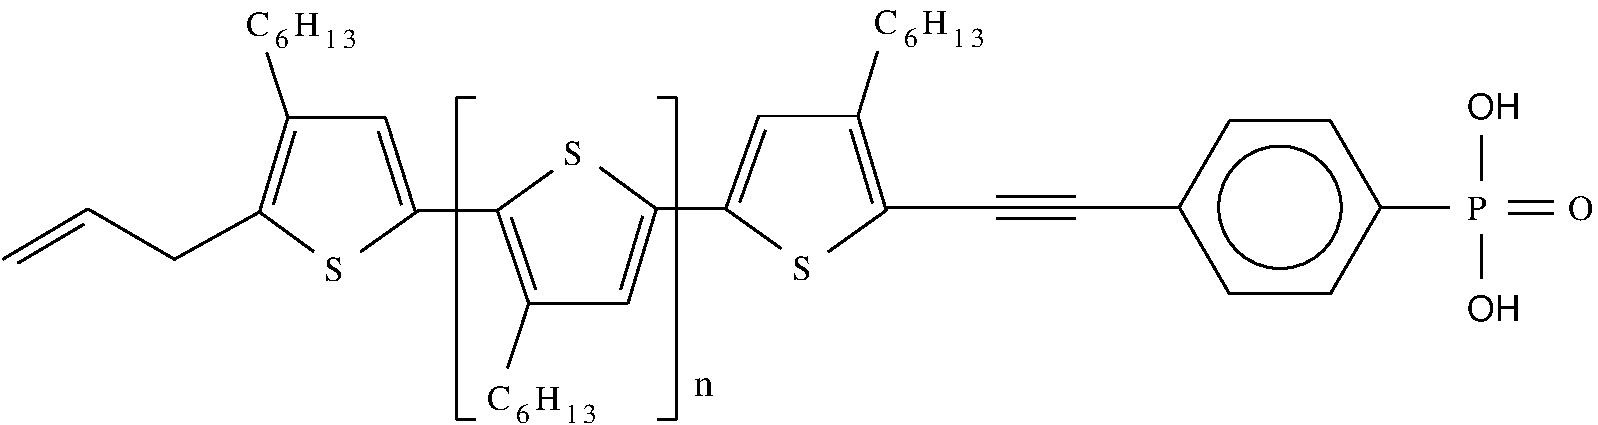
\includegraphics[width=0.7\textwidth]{Immagini_Tesi/pol-finale.pdf}}
\end{figure}
\end{frame}

}
%%%%%%%%%%%%%%%%%%%%%%%%%%%%%%%%%%%%%%%%%%%%%%%%%%%%%%%%%%%%%%%%%%%%%%%%%%%%%%%%%%%%%%%%%%%%%%%%%%%%%%%%%%%%%%%%%%%%%%%%%%%%%%%%%%%%

\diapo{Sistema oggetto di studio}
Riassumendo, la \alert{composizione} del sistema oggetto di studio è:
	\begin{itemize}
	  \item \emph{Quantum dots}: \alert{nanosfere di CdSe} $\phi = 3 - 6$~nm
	  \item Polimero: P3HT \alert{poli(3-esiltiofene) regioregolare monoterminato} con gruppo contenente un \alert{acido fosfonico}
	\end{itemize}
	Il sistema oggetto di studio dovrebbe consentire di ottenere architetture di tipo \alert{\emph{bulk heterojunction}} ovvero film sottili in cui la dispersione si avvicini ad essere bicontinua.
\end{frame}
